Soient ${\cal CC}(G_c)$, l'ensemble des cliques du line-graphe $G_c$ et 
le graphe non orient\'e $G'=(V',E')$ sous-jacent du DAG $G$.

Nous consid\'erons que chaque clique de ${\cal CC}(G_c)$ est un sommet dans $G'$.
Si l'intersection de deux cliques $c_1, c_2 \in {\cal CC}(G_c)$ retourne l'ar\^ete $a_i$  alors nous ajoutons  l'ar\^ete $a_i $ dans $E'$ entre les sommets  $c_1, c_2 \in G'$.
Dans  le cas o\`u un sommet de  $G_c$ n'appartient qu'\`a une seule clique $c \in {\cal CC}(G_c)$, nous ajoute  un nouveau sommet (not\'e $ext\_c$) dans $V'$ puis nous ajoutons une ar\^ete $(ext\_c, c)$ dans $E'$.
Nous obtenons le graphe $G'$ non orient\'e connexe.
Nous utilisons la figure \ref{ExempleGraphesRacinesIsomorphes} pour illustrer la construction de $G'$.
La couverture de corr\'elation de $G_c$ est ${\cal CC}(G_c) = [
 c_1 = \{\{a,b\},\{b,c\},\{b,d\}\}, 
 c_2=\{  \{d,f\},\{f,h\},\{c,f\} \}, 
 c_3 = \{  \{b,c\},\{c,e\},\{c,f\} \}, 
 c_4 = \{  \{c,e\},\{e,g\} \}, 
 c_5 = \{  \{b,d\},\{d,f\} \}]$.
Les sommets du $G'$ sont $V' = \{c_1, c_2, c_3, c_4, c_5\}$.
L'intersection des cliques ci-dessous est non vide et le sommet d'intersection est l'identifiant d'une ar\^ete dans $G'$.
$$
c_1 \cap c_3 = \{b,c\}, ~ 
c_1 \cap c_5 = \{b,d\}, ~ 
c_3 \cap c_2 = \{c,f\}, ~ 
c_3 \cap c_4 =   \{c,e\}, ~ 
c_2 \cap c_5 = \{d,f\}
$$
Pour les sommets de $G_c$ couverts par une seule clique, nous cr\'eons le sommet $ext\_x$ dans $G'$ avec $x$ le nom d'une clique de ${\cal CC}(G_c)$ 
puis nous ajoutons une ar\^ete entre le sommet $ext\_x$ et le sommet de $G'$ correspondant \`a la clique.
Par exemple le sommet $\{a,b\}$ de $G_c$ est couvert par la clique $c_1$. 
Nous relions $ext\_c_1$ de $G'$ avec le sommet $c_1$ de $G'$. 
Nous r\'ep\'etons la m\^eme op\'eration pour les sommets  $\{f,h\}$, $\{e,g\}$ de $G_c$.
Le graphe $G'$ (figure \ref{ExempleGraphesRacinesIsomorphes}(c)) est ainsi construit et est isomorphe au graphe $G$ de la figure \ref{ExempleGraphesRacinesIsomorphes}(a).
% ---- figure graphes racines isomorphe
\begin{figure}[htb!] 
\centering
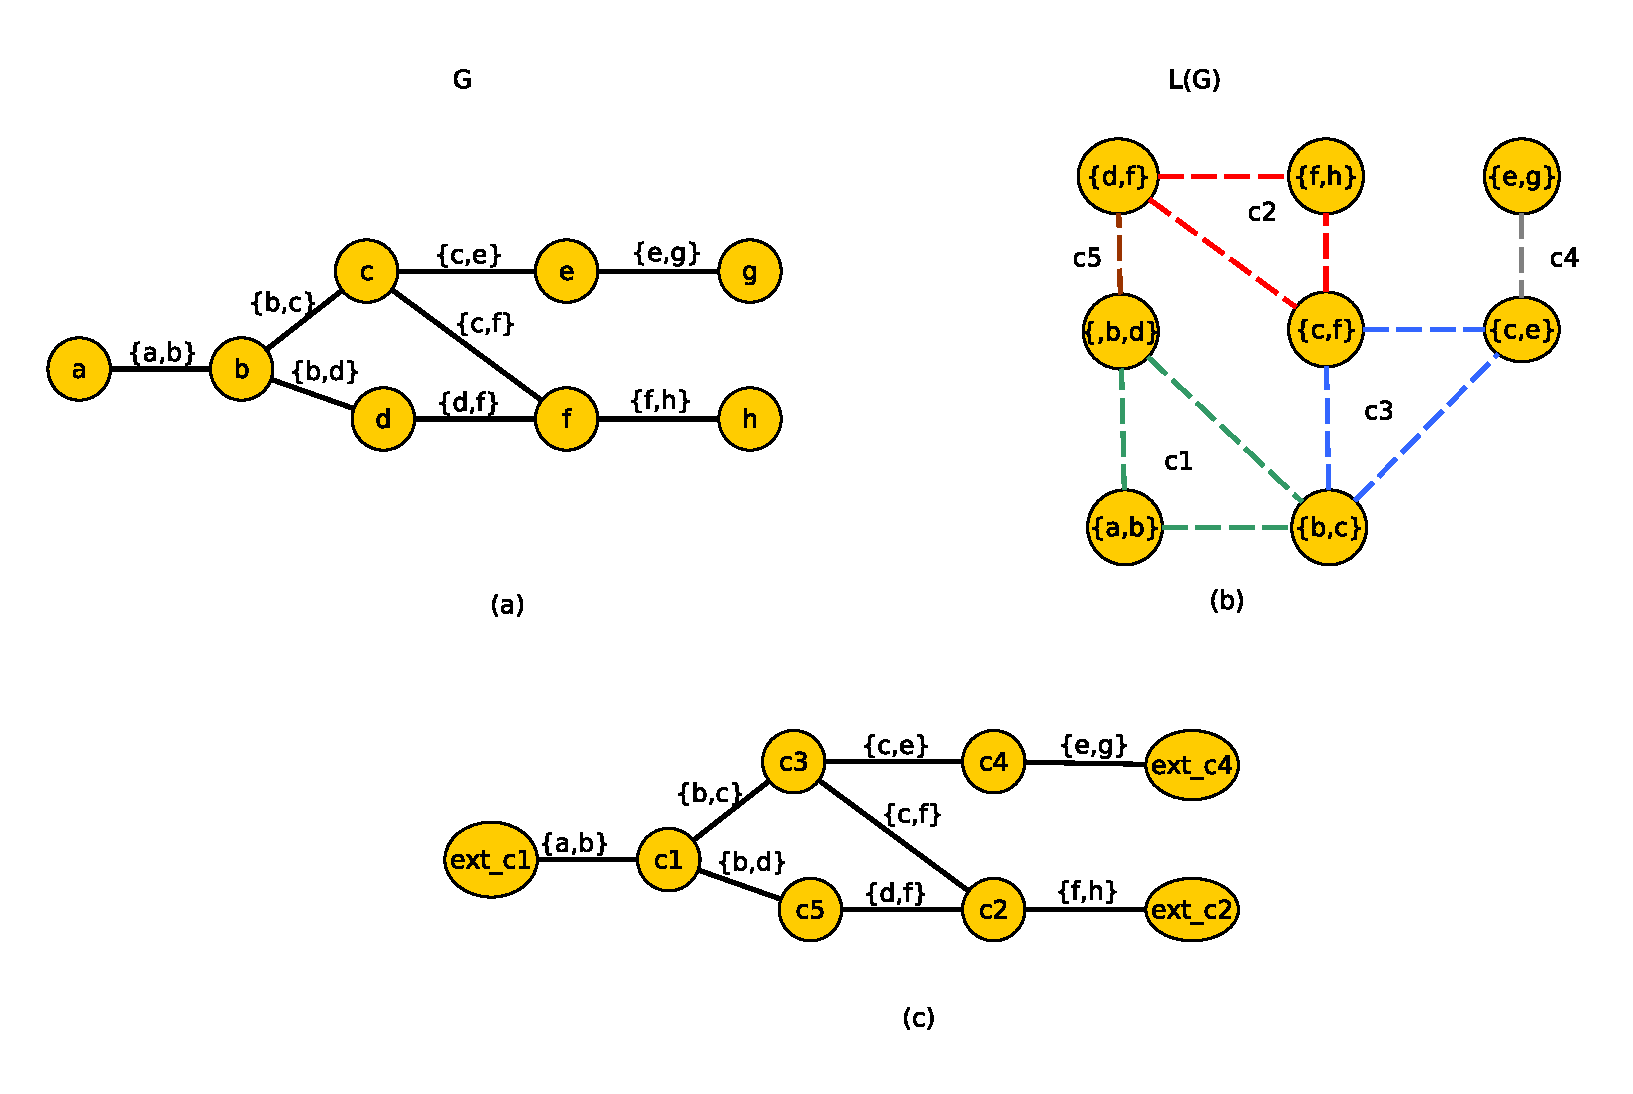
\includegraphics[scale = 0.7]{ExempleGraphesRacinesIsomorphes.eps}
\caption{ Construction de la topologie non orient\'e de $G_c$.
		(a) : r\'eseau initial mod\'elis\'e par $G$.
		(b) : line graphe de $G$.
		(c) : graphe $G'$ reconstruit.
		 }
\label{ExempleGraphesRacinesIsomorphes}
\end{figure}
%\FloatBarrier
% ---- figure exemple correction graphe cellule G_{3,3}

\subsection{Orientation du graphe $G'$}
Nous supposons que le graphe non orient\'e $G'=(V',E')$ sous-jacent au DAG $G$ a d\'ej\`a \'et\'e  obtenu. Nous orientons les ar\^etes de $G'$ afin de d\'ecouvrir  le DAG cible.
 \newline
 
 Soient 
 un sommet $v$, 
 son voisinage $N(v)$ et 
 une bipartition $p(v)$, $s(v)$ de $v$.
 \newline
 Si $Verif-correl (p(v), s(v)) = 1$ alors la partie $p(v)$ est l'ensemble $p(v)$ des arcs entrants de $v$ et  la partie $s(v)$ est l'ensemble $s(v)$ des arcs sortants de $v$.    
Sinon la bipartition n'est pas la bonne et nous testons une autre bipartition.
Nous testons ainsi dans l'ordre de $2^{d(v)}$ bipartitions avec $d(v) = |N(v)|$ dans le pire des cas,.
\newline
Soit une s\'equence $S = v_1, v_2, \cdots, v_k$ de sommets de $G$ telle que 
chaque ar\^ete est incidente \`a $\{v_1, \cdots, v_k\}$ et que  $\{v_1, \cdots, v_{k-1}\}$ n'a pas cette propri\'et\'e.
\newline
Soit $d_i$ le nombre d'ar\^etes liant \`a $v_i$ \`a un sommet  de $V-\{v_1,\cdots, v_{i-1}\}$.
%On determine la couverture. {\bf bizarre} 
\newline
Nous allons prendre dans l'ordre chaque sommet de la s\'equence $S$ et nous allons traiter ses ar\^etes pour trouver une bipartition correcte.
Si une ar\^ete a d\'ej\`a \'et\'e trait\'ee pour un sommet, elle n'est plus prise en compte dans les ar\^etes incidentes des sommets suivants dans la s\'equence $S$.
Le traitement du sommet $v_i$ n\'ecessite $2^{d_i}$ op\'erations et le nombre total d'op\'erations est alors 
$$
 2^{d_1} + 2^{d_2} + \cdots + 2^{d_k}
$$  
Notre probl\`eme  est de trouver une telle liste telle que cette somme est minimum.
L'heuristique est, \`a chaque \'etape, de choisir le sommet tel que 
le nombre d'ar\^etes incidentes non encore trait\'ees est minimum.
Par exemple, on commence par le sommet $v_1$ comme sommet de degr\'ee minimum. 
\`A chaque \'etape, on prend le sommet $v_i$ tel que son degr\'e $d_{v_i}$ est minimum.
\newline 

\vspace{-0.5cm}
Cependant, cette heuristique n'est pas optimale et voici un contre-exemple illustr\'e par la figure \ref{orientationAretesHeuristiqueContreExemple}. \newline
Soit le graphe $H$ compos\'e de $3$ cliques $K_5$ et d'un sommet $v$ ayant une ar\^ete incidente avec un seul sommet dans chaque clique $K_5$.
Le sommet $v$ est de degr\'e minimum. 
Nous consid\'erons $2$ s\'equences de sommets diff\'erents pour d\'enombrer les bipartitions. 
La premi\`ere s\'equence suit l'heuristique et la seconde s\'equence d\'ebute par un sommet de $K_5$ de degr\'e $4$. 
\newline
Soit $c(S)$ la somme des bipartitions possibles.  
En consid\'erant l'heuristique, nous d\'ebutons par $v$. 
Puis le sommet suivant de degr\'e minimum est un sommet de $K_5$. On traite tous les sommets de cette clique $K_5$ avant de passer \`a une autre clique $K_5$.
Le nombre de bipartitions trait\'ees avec  l'heuristique est 
$$
	c(S_H) = 2^3 + 3(  2^4 + 2^3+ 2^2 +2^1) = 98
$$
En consid\'erant la seconde s\'equence, on choisit le sommet de $K_5$ de degr\'e minimum. On traite ce sommet en $2^4$ bipartitions. Le sommet suivant est encore dans cette clique mais le nombre de bipartitions baisse \`a $2^3$.
Apr\`es les deux sommets trait\'es, le nombre de bipartitions est $2^4+2^3$.
On r\'ep\`ete le traitement des sommets jusqu'\`a ce que tous les sommets soient trait\'es avant de passer \`a une autre clique $K_5$. 
Dans cette clique, on reprend \`a nouveau la seconde s\'equence.
Le nombre de bipartitions  trait\'ees avec la seconde s\'equence est 
$$
	c(S_2) = 3(  2^4 + 2^3+ 2^2 +2^1) = 96
$$
Nous remarquons que le nombre de bipartitions avec la seconde s\'equence est minimum.
Cet exemple confirme que la solution de l'heuristique n'est pas minimale car il existe une autre s\'equence de choix de ces sommets (ici la seconde  s\'equence) qui minimise le nombre de bipartitions. 
% ---- figure contre exemple  heuristique orientation aretes 
\begin{figure}[htb!] 
\centering
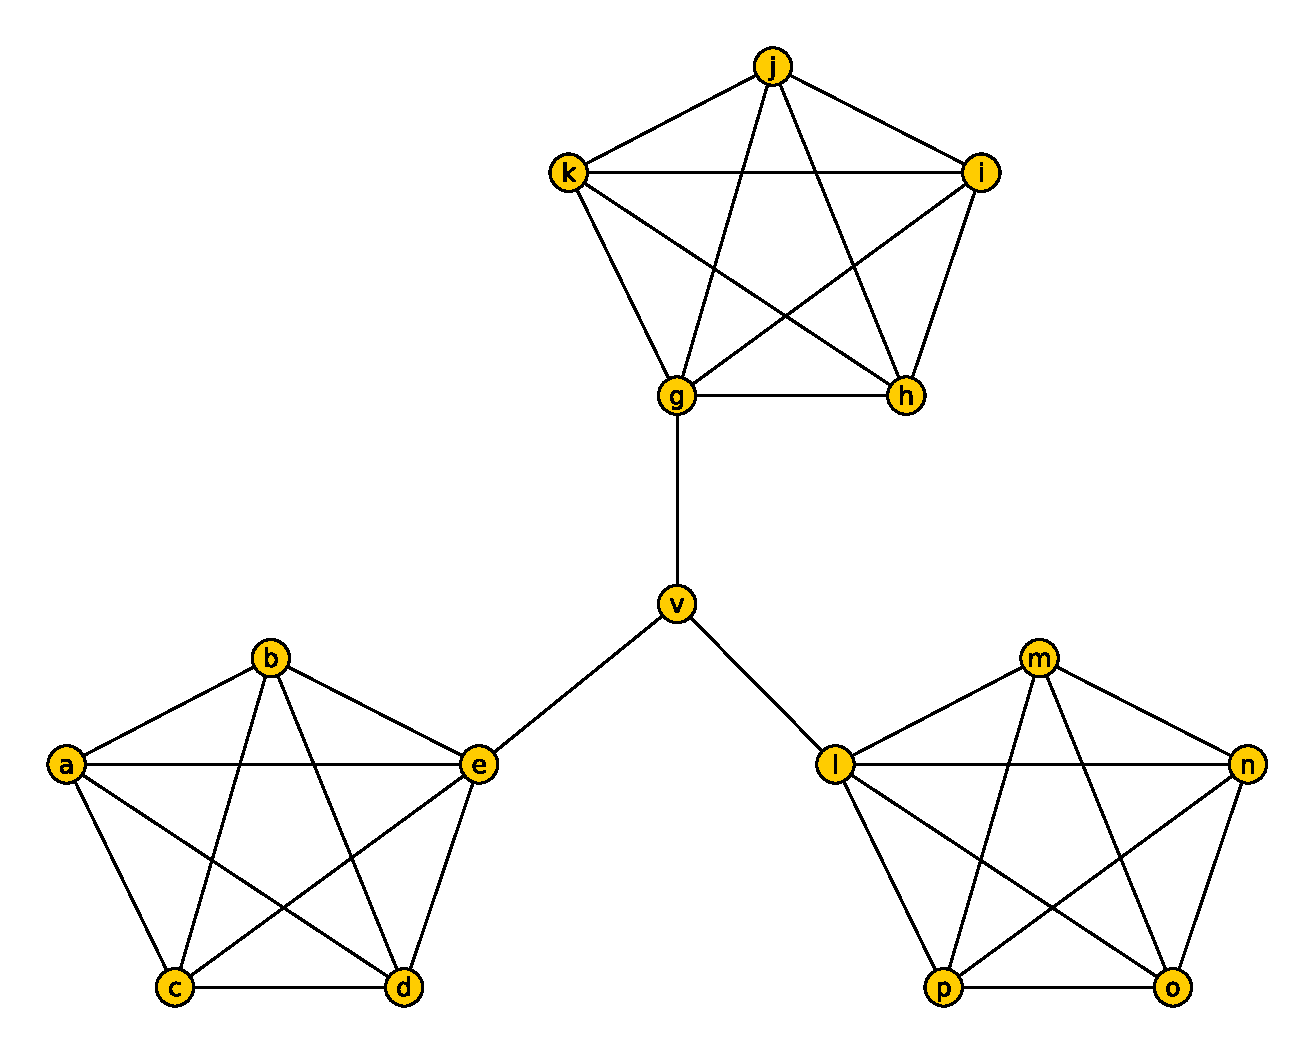
\includegraphics[scale = 0.7]{orientationAretesHeuristiqueContreExemple.eps}
\caption{ Un contre-exemple de l'heuristique choisie pour l'orientation des ar\^etes.
		 On choisit un sommet de degr\'e minimum dans une clique $k_5$. Ensuite, on traite tous les sommets de la clique et on se sert du degr\'e minimum pour choisir les sommets de la s\'equence. Puis on passe \`a une clique et on reprend le traitement jusqu'\`a ce qu'il ne reste plus d'ar\^etes dans une seule clique.
		}
\label{orientationAretesHeuristiqueContreExemple}
\end{figure}
\FloatBarrier
% ---- figure contre exemple  heuristique orientation aretes
%\newline

{\bf Conclusion} : 
l'algorithme d'orientation que nous avons propos\'e choisit le sommet de degr\'e minimum \`a chaque \'etape de l'algorithme et cette solution n'est pas optimale.
Nous conjecturons que la s\'equence $S$ de traitement des sommets est $NP-complet$.


%On le traite avec  $2^3$ bipartitions. Ensuite le sommet suivant de degr\'e minimum est un sommet de $K_5$. On le traite en $2^4$ bipartitions      
%
%
%
%
%Nous supposons que le graphe non-orient\'e $G'=(V',E')$ sous-jacent au DAG $G_c$ ait d\'ej\`a \'et\'e construite. Nous orientons les ar\^etes de $G'$ afin qu'il soit un DAG.
% \newline
% 
%Soit $O = (v_1,v_2, \cdots, v_n)$ la s\'equence de traitement des sommets de $G'$ tel que 
%$d_1 \le d_2 \le \cdots \le d_n$ avec 
%$d_i$ le degr\'e du sommet $v_i$. $d_i$ est aussi le le nombre d'ar\^etes incidentes \`a $v_i$ non trait\'es.
%\newline
%Consid\'erons le premier sommet $v_1$ \`a traiter de $O$ et $N(v_1)$ l'ensemble des  ar\^etes incidentes \`a $v_1$.
%Nous subdivisons $N(v_1)$ en $2$ partitions telles que 
%\begin{itemize}
%	\item $pred(v_1)$ est l'ensemble des ar\^etes pr\'ed\'ecesseurs \`a $v_1$.
%	\item $succ(v_1)$  est l'ensemble des ar\^etes successeurs \`a $v_1$.
%\end{itemize}
%Nous testons cette bipartition $(pred(v_1), succ(v_1))$ avec la fonction $Verif-correl$ \ref{VerifCorrel}.
%Si $Verif-correl$ retourne $Vrai$ alors nous avons orient\'e les ar\^etes incidentes \`a $v_1$.
%Sinon nous testons une autre bipartition.
%Dans le pire des cas, nous testons $2^{d_1}$ bipartitions pour trouver la bonne.
%\newline
%Soit  $(pred(v_1), succ(v_1))$ la bonne bipartition de $v_1$.
%\'Etant donn\'ee que $G'$ est un graphe connexe et que une ar\^ete $a_i$ est form\'ee par les sommets $v_i$ et $v_j$ de $G'$, 
%$a_i$ appartient \`a l'ensemble des successeurs de $v_j$ si $a_i$ a d\'ej\`a \'et\'e trait\'e en pr\'ed\'ecesseur de $v_i$.
%De m\^eme, $a_i$ appartient \`a l'ensemble des pr\'ed\'ecesseurs de $v_j$ si $a_i$ a d\'ej\`a \'et\'e trait\'e en successeur de $v_i$.
%Ainsi, le nombre de bipartitions \`a tester devient moins important au traitement d'un nouveau sommet de $O$.
%En effet, le nombre de bipartitions \`a tester en traitant le sommet  $v_2$ est $2^{d_2}$ et $2^{d_2} \le 2^{d_1}$.
%En traitant le dernier sommet $v_n$ de $O$, nous testons une seule bipartition parce que tous les ar\^etes ont d\'ej\`a \'et\'e trait\'es. Cette bipartition est la bonne et $2^{d_n} = 1$.
%\newline
%Nous d\'eduisons que 
%$$
%1 = 2^{d_n} \le \cdots \le 2^{d_2} \le 2^{d_1}
%$$
%
%L'algorithme d'orientation que nous avons propos\'e choisit le sommet de degr\'e minimum \`a chaque \'etape de l'algorithme et cette solution est minimale.
%Nous conjecturons que la s\'equence $O$ de traitement des sommets est $NP-complet$.
%
%
%
%%% ----
%%% decouverte de topologie du reseau energetique
%%% ----
%%Soient $\cal H$, l'ensemble des cliques de la line-graphe $G_c$ et $G$ le graphe racine de $G_c$. \newline
%%Chaque clique $C_k \in {\cal H}$ correspond \`a un sommet du graphe racine $G$. \newline 
%%Soit $u = \{ENTRANT, SORTANT, NONE\}$, l'ensemble des marquages de chaque ar\^ete tel que les \'etiquettes {\em ENTRANT} et {\em SORTANT} sont associ\'ees respectivement \`a l'ar\^ete $a_i$ entrante et \`a l'ar\^ete $a_j$ sortante du sommet $C_k$.
%%\newline
%%%-- definition de S_1 e S_2
%%Soient $S_1$ et $S_2$ l'ensemble des arcs entrants et sortantes du sommet $C_k$.
%%\begin{equation}
%%S_\alpha = \{ S_{\alpha,i}, \hspace{0.2 em} \forall i \le 2^{card(C_k)+1}  \}
%%\end{equation}
%%avec $i$, le nombre de sous-ensemble de $C_k$ et $\alpha = \{1,2\}$. Le sous-ensemble $S_{\alpha,i}$ peut \^etre  l'ensemble vide $\emptyset$.
%% 
%% %--  ORACLE ou Verif-correl
%% \begin{definition}
%% Soit la clique $C_k$ de la line-couverture {\cal H}.
%% Un couple $(S_1,S_2)$ de sous-ensembles de $C_k$ est {\bf valide} si 
%% \begin{itemize}
%% \item $S_1 \ne S_2$
%% \item $S_1 \cup S_2 = C_k$
%% \item $S_1 \cap S_2 = \emptyset$
%% \end{itemize}
%% \end{definition}
%% 
%% \begin{definition}
%% Soit une fonction bool\'eenne $Verif-correl$ d\'efinit de $S_1 \times S_2 \rightarrow \{0,1\}$, avec le couple valide $(S_1,S_2)$.
%% La fonction $Verif-correl$ renvoie $1$ si et seulement si la loi de conservation autour du sommet $C_k \in G$ est respect\'ee c'est-\`a-dire : 
%% \begin{equation}
%% \forall a_i \in S_1, \forall a_j \in S_2, \sum_{a_i \in S_1} gp_{a_i} - \sum_{a_j \in S_2} gp_{a_j} \le \epsilon
%% \end{equation}
%% avec $\epsilon$ les pertes minimales par effets joules, $gp_{a_i}$ le flot dans l'arc $a_i \in E(G_c)$.
%% \end{definition}
%% 
%% \begin{property}
%% Si $Verif-correl(S_1, S_2) = 1$ alors l'ensemble  $S_1$ est l'ensemble des arcs entrants et  $S_2$ l'ensemble des arcs sortants du sommet $C_k \in G$.
%% \end{property} 
%%Les arcs de $S_1$ et $S_2$ ne concourent pas \`a un sommet $C_k$ lorsque  $Verif-correl(S_1, S_2) = 0$.
%%
%%\begin{theorem}
%%\label{arcsentrantsSortants}
%%%Un arc $a_i$ est soit {\em entrant}, soit {\em sortant} mais jamais les deux.
%%Si un sommet $a_i \in G_c$ appartient \`a deux cliques $C_{k_1}, C_{k_2} \in {\cal H}$ alors 
%%l'arc  $a_i \in E(G_c)$ est soit {\em entrant} de $C_{k_1}$  et {\em sortant} de $C_{k_2}$ ou soit {\em entrant} de $C_{k_2}$  et {\em sortant} de $C_{k_1}$.
%%\end{theorem}
%%
%%\begin{proof}
%%D'apr\`es le th\'eor\^eme \ref{caracteristiquesLinegraphes}, le sommet $a_i$ appartient \`a deux cliques $C_{k_1}$ et $C_{k_2}$ au maximum. 
%%Cela implique qu'il existe une ar\^ete entre les sommets $C_{k_1}$ et $C_{k_2}$ dans $G$.
%%Soient $S_1, S_2 \subset C_{k_1}$ et $S_3, S_4 \subset C_{k_2}$ telles que $Verif-correl(S_1, S_2) = 1$ et $Verif-correl(S_3, S_4) = 1$.
%%Comme  $S_1 \cap S_2 = \emptyset$, $S_3 \cap S_4 = \emptyset$ et aussi  $C_{k_1} \cap C_{k_2} = \{a_i\}$, on a quatre choix possibles :
%%$a_i \in S_1 \cap S_3$, $a_i \in S_1 \cap S_4$, $a_i \in S_2 \cap S_3$, $a_i \in S_2 \cap S_4$.
%%\newline
%%Si $a_i$ est entrant \`a $C_{k_1}$ et sortant \`a  $C_{k_2}$ alors $a_i \in S_1 \cap S_3$ ou  $a_i \in S_2 \cap S_4$. 
%%On en d\'eduit qu'il existe une boucle sur le sommet $C_{k_1}$ et $C_{k_2}$. 
%%Cela est impossible parce que $G$ est un $DAG$. 
%%\newline
%%Ainsi si $a_i$ est entrant \`a $C_{k_1}$ alors $a_i \in S_2 \cap S_3$ ou  si $a_i$ sortant \`a $C_{k_2}$  alors $a_i \in S_1 \cap S_4$. 
%%\end{proof}
%%
%%consid\'erons l'ensemble $A$ des cliques $C_j$ tel que $card(C_j) = min\{ card(C_k), C_k \in {\cal H}\}$ et la fonction  $Z$ qui retourne l'\'etiquette d'un sommet dans une clique. $Z$ est d\'efinie comme suit:
%%$E \times {\cal H} \rightarrow \{ENTRANT, SORTANT, NONE\} $.
%%\newline
%%Soit la fonction $f$ d\'efinie sur $ V(G_c) \times A \rightarrow \{0,1\}$ retournant $1$ si le sommet $a_i^u$ ne poss\`ede aucune \'etiquette c'est-\`a-dire labellis\'e \`a $None$.
%%$$ f(a_i^u, C_j) = \begin{cases} 1 ~~~ si ~~~ Z(a_i^u, C_j) \ne NONE \\ 0 ~~~ sinon \end{cases}$$.
%%La fonction $MA$ calcule le nombre de sommets labellis\'e dans une clique $C_k$.
%%$$MA(C_k) =  \sum_{a_i^u \in C_k} f(a_i^u,C_k) $$
%%Soient la clique $C_m$ telle que  $MA(C_m) = max\{ MA(C_j), C_j \in A\}$ et $B$ l'ensemble des sommets de la clique $C_m$ tel que $Z( a_j^v, C_m) == NONE, ~ \forall ~ a_j^v \in B$. 
%%
%%
%%%nommer l'algorithme
%%\begin{algorithm}[!ht]
%%\caption{Decouverte\_graphe\_racine}
%%\noindent DEBUT\\
%%\noindent 1. Initialisation des \'etiquettes des sommets $a_i$ de $G_c$, et $C_k \in {\cal H}$ \\
%%\noindent $Z( C_k, a_i^u) = None$ \\
%%~2. \indent {\bf Tant que} il existe une  ar\^ete de $G_c$ ($E(G_c)$) \\
%%	\indent~~~~~~{\bf Faire}\\
%%~3.		\indent~~~~~~~~choisir $A = \{C_j , card(C_j) = min\{ card(C_k), C_k \in {\cal H} \}\}$ \\
%%~4.		\indent~~~~~~~~choisir $C_k$ tel que $MA(C_k) = max\{ MA(C_j), C_j \in A\} $ \\
%%~5.       	\indent~~~~~~~~{\bf Si} il existe $S_1$ et $S_2$ tel que $S_1 \cap S_2 = \emptyset $ et $S_1 \cup S_2 = C_k $ et $Verif-correl(S_1, S_2 )= 1 $ \\
%%~6.	       	\indent~~~~~~~~~~~~{\bf alors}\\
%%~7.	       	\indent~~~~~~~~~~~~ $S_1^k = sommets\_marques(S_1, Z)(^1)$; \\
%%~8.	       	\indent~~~~~~~~~~~~ $S_2^k = sommets\_marques(S_2, Z)$; \\
%%~9.		\indent ~~~~~~~~~~~~{\bf Pour tout} $a_i^K \in S_1 - S_1^k$ {\bf Faire} \\
%%~10.		\indent ~~~~~~~~~~~~~ $Z(C_k, a_i^K) = ENTRANT$ \\
%%~11.		\indent ~~~~~~~~~~ {\bf Pour tout} $a_i^K \in S_2 - S_2^k$ {\bf Faire} \\
%%~12.		\indent ~~~~~~~~~~~~~ $Z(C_k, a_i^K) = SORTANT$ \\
%%~13.		\indent~~~~~~~~~~ $E(G_{c}) =  E(G_c)  - E(G_c[C_k])$ \\
%%~14.		\indent~~~~~~~~~~ ${\cal H} =  {\cal H}  - C_k$ \\
%%~15.       	\indent~~~~~~~~{\bf FinSi} \\
%%~16. \indent {\bf FinTant que} \\
%%~17. \indent {\bf Pour tout} $a_i^u \in V(G_c)$ {\bf Faire} \\
%%~18. \indent ~~~ $C_1, C_2$ = $Couverture\_Cliques(a_i^u)(^2)$\\
%%~19. \indent ~~~ {\bf Si } $C_1 \neq \emptyset$ et $C_2 \neq \emptyset$ {\bf Alors} \\
%%~20. \indent ~~~~~~  {\bf Si}  $Z(C_1, a_i^u) == SORTANT$ {\bf Alors} \\
%%~21. \indent ~~~~~~~~~~~~ $Mat(C_1)$ += $C_2$ $(^3)$ \\  
%%~22. \indent ~~~~~~  {\bf Fin Si} \\
%%~23. \indent ~~~~~~  {\bf Si}  $Z(C_2, a_i^u) == SORTANT$ {\bf Alors} \\
%%~24. \indent ~~~~~~~~~~~~ $Mat(C_2)$ += $C_1$ $(^3)$ \\  
%%~25. \indent ~~~~~~  {\bf Fin Si} \\
%%~26. \indent ~~~ {\bf Fin si} \\
%%~27. \indent ~~~ {\bf Si } $C_1 \neq \emptyset$ et $C_2 == \emptyset$ {\bf Alors} \\
%%~28. \indent ~~~~~~  {\bf Si}  $Z(C_1, a_i^u) == ENTRANT$ {\bf Alors} \\
%%~29. \indent ~~~~~~~~~~~~ $Mat(EXT\_a_i^u)$ += $C1$ $(^3)$\\  
%%~30. \indent ~~~~~~  {\bf Fin Si} \\
%%~31. \indent ~~~~~~  {\bf Si}  $Z(C_1, a_i^u) == SORTANT$ {\bf Alors} \\
%%~32. \indent ~~~~~~~~~~~~ $Mat(C_1)$ += $EXT\_a_i^u$ $(^3)$ \\  
%%~33. \indent ~~~~~~  {\bf Fin Si} \\
%%~34. \indent ~~~ {\bf Fin si} \\
%%~35. \indent {\bf Fin Pour} \\
%%~36. \noindent {\bf Return} Mat\\
%%\noindent FIN\\
%%\end{algorithm}
%%
%%\FloatBarrier
%%$^1$ : Cette fonction retourne les sommets de l'ensemble $S_1$ labellis\'es \`a $ENTRANT$ et $S_2$ labellis\'es \`a $SORTANT$. Initialement, Ces sommets sont \'etiquett\'es \`a $NONE$.
%%
%%$^2$ : Cette fonction renvoie les cliques couvrantes une ar\^ete $a_i^u$ avec $C_1 \ne \emptyset$. Si $a_i^u$ est couvert par une clique alors $C_2 = \emptyset$.
%%
%%$^3$ : $EXT\_a_i^u$ est un sommet du graphe racine $G$.
%%\newline
%%
%%L'algorithme {\em Decouverte\_graphe\_racine} d\'ebute par l'initialisation des sommets de $G_c$ \`a $''None''$.
%%Tant qu'il existe une ar\^ete dans notre line-graphe $G_c$, on choisit la plus petite clique $C_k$ dans laquelle le nombre de sommets labellis\'es est maximal quelque soit le label {\em ENTRANT} et {\em SORTANT} (lignes $3-4$).
%%On partitionne la clique $C_k$  en deux sous-ensembles valides $S_1$ et $S_2$ tels que $S_1$ et $S_2$ correspondent, respectivement, \`a l'ensemble des arcs entrants et sortants du graphe racine $G$.
%%Les sommets labellis\'es de $S_1$ not\'es $S_1^k$ portent l'\'etiquette $ENTRANT$ tandis que ceux labellis\'es en $''SORTANT''$ sont not\'es $S_2^k$ (lignes $6-12$). 
%%Ensuite nous mettons \`a jour l'ensemble des ar\^etes et la line-couverture  $\cal C$ de $G_c$ (lignes $13-14$). 
%%\newline
%%Une fois termin\'e l'orientation des ar\^etes de $G$ qui  sont les sommets labellis\'es du line-graphe $G_c$ (lignes $2-16$), nous construisons la liste d'adjacence de chaque sommet de $G$ (lignes $17-36$).
%%Nous recherchons la couverture d'un sommet $a_i^u$ de $G_c$.
%%\newline 
%%Si le sommet  $a_i^u$ est couvert par une seule clique alors $C_2 = \emptyset$. Dans ce cas, cela signifie qu'il existe un arc entre le sommet $C_1$ et le sommet $EXT\_a_i^u$ que nous avons cr\'ee. Cet arc a pour extr\'emit\'e initiale $C_1$ si $a_i^u$ est labellis\'e par $SORTANT$ sinon pour extr\'emit\'e initiale $EXT\_a_i^u$ si $a_i^u$ est labellis\'e par $ENTRANT$ (lignes $27-34$).
%%\newline
%%Dans le cas o\`u le sommet $a_i^u$ est couvert par deux cliques non vides $C_1, C_2$, nous ajoutons un arc entre ces deux cliques.
%%D'apr\'es le th\'eor\`eme  \ref{arcsentrantsSortants}, nous d\'efinissons  $C_1$ comme extr\'emit\'e initiale de cet arc si $a_i^u$ est labellis\'e par $SORTANT$ dans cette clique $C_1$. Dans le cas o\`u $a_i^u$ est labellis\'e par $SORTANT$ dans cette clique $C_2$, $C_2$ est l'extr\'emit\'e finale de cet arc (lignes $19-26$).
%%%D'apr\'es le th\'eor\`eme  \ref{arcsentrantsSortants} stipulant qu'un sommet de $G_C$ est $''ENTRANT''$ de $C_1$ et $''SORTANT''$ de $C_2$ et vice-versa, nous d\'efinissons  $C_1$ comme extr\'emit\'e initiale de cet arc si $a_i^u$ est labellis\'e par $SORTANT$ dans cette clique $C_1$ sinon $C_2$ si $a_i^u$ est labellis\'e par $SORTANT$ dans cette clique $C_2$ (lignes $19-26$).
%%
%%\subsection{Complexit\'e de l'algorithme {\em Decouverte\_graphe\_racine} }
%%
%%La fonction $Couverture\_Cliques$ a une complexit\'e constante $O(1)$ alors que la complexit\'e de la  fonction $sommets\_marques$ depend du nombre de sommets dans $S_1$. Dans le pire des cas, sa complexit\'e est $O(n)$ avec $n = E(G)$ le nombre  d'arcs de $G$. Donc les lignes $17-35$ s'ex\'ecutent en $O(n)$ dans le pire des cas. 
%%\newline
%%Consid\'erons une line-couverture ${\cal H}$  de taille $K$,  une clique $C_i \in {\cal H}$ de taille $p_i$ et $k_i$ le nombre de sommets marqu\'es dans $C_i$. 
%%\newline
%%Le nombre de couples valides $(S_1,S_2)$ pour la clique $C_i$ avec $k_i$ sommets marqu\'es est $2^{p_i -k_i}$. 
%%Au traitement de la premi\`ere clique de ${\cal C}$ de taille minimale $C_1$, il existe $0$ sommet marqu\'e. Le co\^ut $R_{cv_1}$ de couples valides est $R_{cv_1} = 2^{p_1}$.
%%Au traitement de la seconde clique $C_2$, il existe $k_2 \ge 0$ et son co\^ut est  $R_{cv_2} = 2^{p_2 - k_2}$.
%%Il existe une clique $C_\alpha$ \`a partir de laquelle $k_\alpha > 0, \alpha \le K$.
%%On remarque que $p_\alpha - k_\alpha$ est d\'ecroissant car $k_\alpha$ augmente apr\`es chaque traitement de cliques. 
%%Cela signifie qu'\`a la selection de la derni\`ere clique $C_k$, son co\^ut  est de $R_{cv_K} = 1$. 
%%Le co\^ut est decroissant \`a chaque traitement c'est-\`a-dire 
%%$$2^{p_{\alpha} - k_{\alpha}} \ge 2^{p_{\alpha+1} - k_{\alpha+1}} \ge \cdots \ge 2^{p_K - k_K}$$ 
%%Le co\^ut des couples valides de ${\cal H}$ est 
%%$$R_{cv} = O(2^\gamma), \gamma = max\{card(C_i), \forall C_i  \in \{C_1, \cdots, C_\alpha\} \}$$
%%car il depend de la clique $C_i \in \{C_1, \cdots, C_\alpha\} \subset {\cal H}$.
%%\newline
%%Le co\^ut des lignes $3-4$ depend de $p_i$ et $K$ ($O(p_i) + O(K)$) et celui des lignes $7-14$ est de $O(p_i^2)$.
%%\newline
%%Soit le co\^ut $R$ de la boucle  {\em Tant que}. Il est de 
%%$$ R = O(p_i) + O(K) + O(p_i^2) + O(2^\gamma) \simeq O(2^\gamma)$$
%%
%%La complexit\'e de {\em Decouverte\_graphe\_racine} est {\em pseudo-exponentielle} car l'exposant $\gamma$ est la taille d'une clique de taille interm\'ediaire.
%%
%%%Consid\'erons les instructions dans le boucle {\em Tant que}, $K$ le cardinal de ${\cal C}$ et $p$ le cardinal de la clique de taille minimale de ${\cal C}$ c'est-\`a-dire $card(A) = p$. 
%%%\newline
%%%$R_i$ est le co\^ut de la boucle {\em Tant que} au traitement de la $i^eme$ clique de $G_C$ et $C\_oracle$ le co\^ut de la fonction $ORACLE$.
%%%S\'electionnons le premier clique de $G_C$. Son co\^ut est :
%%%$$R_1 = p \times C_oracle(S_{1p}, S_{2p}) $$.
%%%Le co\^ut  du deuxi\`eme sommet est :
%%%$$R_2 = p \times C_oracle(S_{1p}, S_{2p})  + (p-1) \times C_oracle(S_{1p-1}, S_{2p-1})  $$.
%%%Le co\^ut des $n$ sommets de $G_C$ est :
%%%$$R_K = \sum_{k = 0}^{K-1} (p-k) \times C_oracle(S_{1p-k}, S_{2p-k})$$
%%%
%%%La particularit\'e de l'ORACLE est que pour $k \ge p$, tous les sommets de la clique $C_k$ sont labellis\'es entrainant qu'on ne genere aucuns sous-ensembles de $C_k$. Cela implique que  $C_oracle(S_{1p-k}, S_{2p-k}) = 1$. \newline
%%%Cela revient \`a dire que le co\^ut $R_K$ est d\'ecroissant en fonction de $K$. \newline
%%%G\'en\'erer tous  sous-ensembles de $C_k$ de taille $p$ est une combinaison de 
%%%$card(P(E)) = 2^{p}$ et toutes les paires de $P(E)$ vaut au pire des cas $\frac{2^p * (2^p - 1)}{2}$. 
%%%Alors  le  cout  $C_oracle(S_{1p}, S_{2p}$ est $O(2^p)$ ===> FAUX
%%%%%%% A discuter avec SERGES ---> trouver le nombre de tuples provenant des sous ensembles  de C_k de taille $p$
%%%Donc le co\^ut de $R_K$ est  
%%%$$R_K = p \times O(2^p) + (p-1) \times O(2^{(p-1)}) + \cdots + 1 \times O(2^0)$$
%%%$$ R_K $$
%%%PAS FINI
%%
%%
